\section{解的含义}
\label{sec:pdeprob-solutions}

到目前为止，“$u$满足方程”都是指把导数算出来、逐点代入。前面几个例子已经暴露了这种理解的局限：折线初值的折角在波动方程中一直存在，初值和边值不相容时输运方程的解带一条间断线。这些函数是不是解？要回答这个问题，就要明确“满足方程”的方式。

\paragraph{经典解}
最直接的要求是方程涉及的导数都存在且连续，方程逐点成立，初边值也逐点取到。

\begin{definition}[经典解]
\label{def:pdeprob-classical}
设$\Omega$是有界开集。Poisson方程$-\Delta u=f$配边值$u=g$的\term{经典解}（classical solution）是满足下列条件的函数：$u\in C^{2}(\Omega)\cap C(\overline{\Omega})$，在$\Omega$内每一点$-\Delta u=f$，在$\partial\Omega$上每一点$u=g$。对热方程问题~\eqref{eq:pdeprob-heat-ibvp}，经典解要求$u$对$\bm{x}$二阶、对$t$一阶连续可微于$\Omega\times(0,T]$，在$\overline{Q}$上连续，方程和初边值逐点成立。
\end{definition}

定义中的两层要求分工不同：内部的光滑性让方程有意义，到边界的连续性让边值有意义。热方程不要求光滑到$t=0$，正是为了容纳第~\ref{sec:pdeprob-initial}小节中的折线初值。

经典解的概念在两种情况下不够用：数据本身粗糙，或者解在演化中自己失去光滑性。下面逐一看。

\paragraph{粗糙的源项}
在$(0,1)$上考虑$-u''=f$，$u(0)=u(1)=0$，其中源项只在中间一段加热：
\begin{equation}
  f(x)=\begin{cases}4,&1/4<x<3/4,\\0,&\text{其他}.\end{cases}
  \label{eq:pdeprob-step-source}
\end{equation}
若$u\in C^{2}$，$u''$连续，但$u''=-f$在$x=1/4$处跳跃，所以经典解不存在。可是这根棒有确定的稳态温度，问题出在我们对“解”的要求太高。

分段把这个温度算出来。由对称性，$u'(1/2)=0$，所以在中段$u'(x)=-4(x-1/2)$，到左分界点时$u'(1/4)=1$。在$(0,1/4)$上$u''=0$，$u'$恒为$1$，由$u(0)=0$得
\[
  u(x)=x,\qquad 0\leq x\leq\frac14.
\]
中段积分一次得$u(x)=C-2(x-1/2)^{2}$，由$x=1/4$处连续，$C-\frac18=\frac14$，于是
\[
  u(x)=\frac38-2\Bigl(x-\frac12\Bigr)^{2},\qquad \frac14\leq x\leq\frac34.
\]
右段由对称性得$u(x)=1-x$。

这个函数在图~\ref{fig:pdeprob-weak-piecewise}中是一条光滑的曲线，$u$和$u'$都连续，只有$u''$在两个分界点跳跃。除这两点外方程逐点成立。我们希望有一种“解”的定义，能把它算进去，又不至于什么都算进去。

\begin{BookInlineFigure}
  \centering
  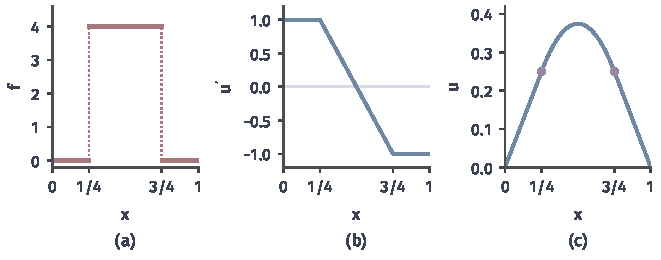
\includegraphics[width=112.0mm]{figures/06-differential-equations/02-partial-differential-equations/matplotlib/pdeprob-weak-piecewise/figure.pdf}
  \caption{跳跃源项下的解。(a)源项$f$，在$1/4$和$3/4$处跳跃。(b)$u'$连续，折点处$u''$跳跃。(c)$u$，紫点标出两个分界点，$u(1/2)=3/8$。}
  \label{fig:pdeprob-weak-piecewise}
\end{BookInlineFigure}

\paragraph{用测试函数检验}
把逐点检验换成加权平均的检验。逐点检验好比用一根无限细的探针逐点测量，而现实的探针总有一定宽度，读到的是附近的加权平均。两个函数相等，既可以逐点比较，也可以用所有光滑探针读数比较，后者不需要任何点上的导数。

设$\varphi$是\term{测试函数}（test function），即在$\Omega$内紧支撑的无穷次可微函数，全体记作$C_c^{\infty}(\Omega)$。若$u$是经典解，把$-\Delta u=f$乘以$\varphi$并在$\Omega$上积分，由分部积分得到
\[
  \int_\Omega\nabla u\cdot\nabla\varphi\,\mathrm{d}\bm{x}=\int_\Omega f\varphi\,\mathrm{d}\bm{x}.
\]
边界项因为$\varphi$在边界附近为零而消失。这个等式只含$u$的一阶导数，导数被挪了一阶到探针上。

把一阶导数也放宽，就要用到弱导数。设局部可积函数$w$对所有测试函数满足
\[
  \int_\Omega u\,\partial_{x_i}\varphi\,\mathrm{d}\bm{x}=-\int_\Omega w\,\varphi\,\mathrm{d}\bm{x},
\]
就称$w$是$u$的弱导数，这个$w$在几乎处处意义下唯一。详细的定义和性质可参考\BookChapterRef{chap:smoothing-weak-derivatives}{卷四第7章“光滑逼近与弱导数”}。

$H^{1}(\Omega)$由本身及各弱导数都属于$L^{2}(\Omega)$的函数组成，$H_0^{1}(\Omega)$是$C_c^{\infty}(\Omega)$在$H^{1}$范数下的闭包，在有界Lipschitz区域上恰好是边界迹为零的函数。这些空间的完备性、迹和嵌入性质可参考\BookChapterRef{chap:sobolev-spaces}{卷四第21章“Sobolev空间”}。

\begin{definition}[Poisson方程的弱解]
\label{def:pdeprob-weak-poisson}
设$\Omega\subset\mathbb{R}^{d}$是有界开集，$f\in L^{2}(\Omega)$。若$u\in H_0^{1}(\Omega)$满足
\begin{equation}
  \begin{gathered}
    a(u,v)=\int_\Omega fv\,\mathrm{d}\bm{x},\qquad\forall v\in H_0^{1}(\Omega),\\
    a(u,v)=\int_\Omega\nabla u\cdot\nabla v\,\mathrm{d}\bm{x},
  \end{gathered}
  \label{eq:pdeprob-weak-form}
\end{equation}
则称$u$是零边值Poisson问题的\term{弱解}（weak solution），式~\eqref{eq:pdeprob-weak-form}称为它的\term{弱形式}（weak formulation）。
\end{definition}

定义的三个成分各有作用。要求$u\in H^{1}$，式~\eqref{eq:pdeprob-weak-form}左边才有意义；要求$u\in H_0^{1}$，把零边值写进了解所在的空间；让$v$取遍$H_0^{1}$而非只取测试函数，并没有增加要求，因为测试函数在其中稠密、等式两边对$v$连续。

分段例子的$u$是弱解。$u$连续可微且在两端为零，所以$u\in H_0^{1}(0,1)$。对测试函数$\varphi$，把积分分成三段分别分部积分：
\[
  \int_0^{1}u'\varphi'\,\mathrm{d}x
  =\sum_{\text{三段}}\Bigl(\bigl[u'\varphi\bigr]-\int u''\varphi\,\mathrm{d}x\Bigr).
\]
$u'$在两个分界点连续，相邻两段的端点项互相抵消，$\varphi$在$0,1$处为零，端点项全部消失。各段内$-u''=f$，于是
\[
  \int_0^{1}u'\varphi'\,\mathrm{d}x=\int_0^{1}f\varphi\,\mathrm{d}x.
\]

弱解的要求并不是“几乎处处满足方程”。在$(0,1)$上取$f=0$，考虑折线$u=\min\{x,1-x\}$，除$x=1/2$外$u''=0$，两端也为零。它是不是$-u''=0$的弱解？取测试函数$\varphi$，同样分段，$u'$在$(0,1/2)$上是$1$，在$(1/2,1)$上是$-1$：
\[
  \int_0^{1}u'\varphi'\,\mathrm{d}x
  =\int_0^{1/2}\varphi'\,\mathrm{d}x-\int_{1/2}^{1}\varphi'\,\mathrm{d}x
  =2\varphi\Bigl(\frac12\Bigr).
\]

结果不为零，所以折线不是弱解：探针读出了折点。这个折点实际上是一个集中在$x=1/2$、强度为$2$的点热源，第~\ref{sec:pdeprob-types}节的点源解就是这一函数的一半。

图~\ref{fig:pdeprob-kink-test}取一个具体的光滑探针演示，(b)中$u'\varphi'$在两侧都是正的，面积加起来等于$2\varphi(1/2)=2$。“几乎处处”忽略了一点上发生的事，而测试函数不会。

\begin{BookInlineFigure}
  \centering
  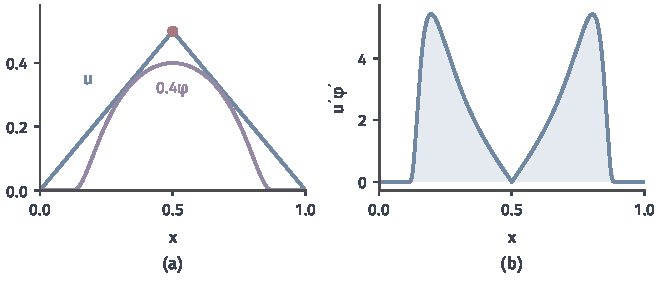
\includegraphics[width=112.0mm]{figures/06-differential-equations/02-partial-differential-equations/matplotlib/pdeprob-kink-test/figure.pdf}
  \caption{探针读出折点。(a)折线$u=\min\{x,1-x\}$（蓝，红点为折点）与测试函数$\varphi(x)=\exp(1-1/(1-r^2))$，$r=(x-\frac12)/0.4$（紫，图中缩放$0.4$倍）。(b)$u'\varphi'$，阴影面积的数值积分为$2.000$，等于$2\varphi(\frac12)$。}
  \label{fig:pdeprob-kink-test}
\end{BookInlineFigure}

弱解是经典解的推广，而不是另一种东西。下面的定理说明，函数足够光滑时两者一致。

\begin{theorem}[弱解与经典解的相容]
\label{thm:pdeprob-weak-classical}
设$\Omega$是有界Lipschitz区域，$f\in C(\overline{\Omega})$，$u\in C^{2}(\overline{\Omega})$且在$\partial\Omega$上$u=0$。则$u$是经典解，当且仅当$u$满足弱形式~\eqref{eq:pdeprob-weak-form}。
\end{theorem}

\begin{proof}
$u$连续可微到边界且边界值为零，所以$u\in H_0^{1}(\Omega)$。对$v\in C_c^{\infty}(\Omega)$，由乘积法则，
\[
  \nabla\cdot(v\nabla u)=\nabla v\cdot\nabla u+v\Delta u.
\]
$v$在边界附近为零，由散度定理，左边的积分为零，于是
\[
  \int_\Omega\nabla u\cdot\nabla v\,\mathrm{d}\bm{x}=-\int_\Omega v\,\Delta u\,\mathrm{d}\bm{x}.
\]

若$u$是经典解，右边等于$\int_\Omega fv\,\mathrm{d}\bm{x}$，对测试函数成立。式~\eqref{eq:pdeprob-weak-form}两边都是$v$在$H^{1}$范数下的连续线性泛函，由稠密性，等式对全部$v\in H_0^{1}(\Omega)$成立。

反过来，若弱形式成立，则对任意测试函数$v$有
\[
  \int_\Omega(-\Delta u-f)\,v\,\mathrm{d}\bm{x}=0.
\]
$-\Delta u-f$连续。若它在某点为正，取在该点附近非负、不恒为零的测试函数$v$，积分为正，矛盾；为负时同理。所以$-\Delta u=f$在$\Omega$内处处成立。
\end{proof}

\paragraph{演化产生的间断}
第二种情况更棘手：数据没有间断，解却在有限时间内失去光滑性。考虑守恒律$\partial_tu+\partial_x(u^{2}/2)=0$，即拟线性方程$\partial_tu+u\,\partial_xu=0$，通常称为Burgers方程。沿直线$x=x_0+u_0(x_0)t$，
\[
  \frac{\mathrm{d}}{\mathrm{d}t}u(x_0+u_0(x_0)t,t)=\partial_tu+u_0(x_0)\partial_xu=0.
\]
所以$u$沿这条直线保持初值$u_0(x_0)$，初值大的点跑得快。

取初值
\begin{equation}
  u_0(x)=\begin{cases}1,&x<0,\\1-x,&0\leq x\leq1,\\0,&x>1.\end{cases}
  \label{eq:pdeprob-burgers-ramp}
\end{equation}
由$x=x_0+(1-x_0)t$解出$x_0=(x-t)/(1-t)$，在$t<1$时得到
\[
  u(x,t)=\frac{1-x}{1-t},\qquad t\leq x\leq1.
\]
这时$\partial_xu=-1/(1-t)$，$t\to1$时斜率趋于无穷。图~\ref{fig:pdeprob-burgers-crossing}(a)中，从$[0,1]$出发的直线全部在$(1,1)$汇聚；(b)中坡面越来越陡，$t=1$时成为垂直的台阶。此后沿直线算出的值成为多值，方程必须换一种读法。斜坡的两个折角只是为了算得出显式解，把它磨成无穷次可微的初值，坡面同样会在有限时间变成垂直。

\begin{BookInlineFigure}
  \centering
  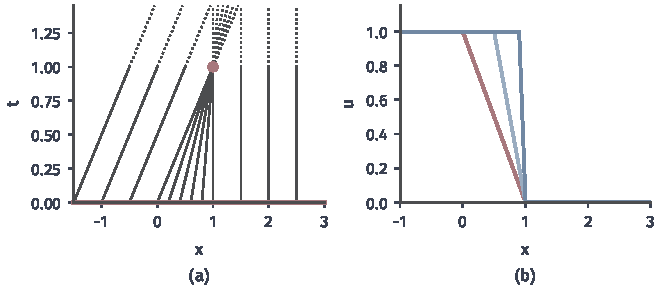
\includegraphics[width=112.0mm]{figures/06-differential-equations/02-partial-differential-equations/matplotlib/pdeprob-burgers-crossing/figure.pdf}
  \caption{Burgers方程的斜坡初值。(a)从初始线（红）出发的直线$x=x_0+u_0(x_0)t$（深灰），在红点$(1,1)$汇聚，虚线部分表示相交后已无法继续沿用。(b)解的形状，红线为$t=0$，蓝色由浅到深为$t=0.5,0.9$。}
  \label{fig:pdeprob-burgers-crossing}
\end{BookInlineFigure}

同样的办法可以用在这里，但必须从守恒形式出发。设$u$是光滑解，把$\partial_tu+\partial_xF(u)=0$乘以$\varphi\in C_c^{\infty}(\mathbb{R}\times[0,\infty))$，在$\mathbb{R}\times(0,\infty)$上积分并分部积分，所有导数都转到$\varphi$上：
\begin{equation}
  \int_0^{\infty}\!\!\int_{\mathbb{R}}\bigl(u\,\partial_t\varphi+F(u)\,\partial_x\varphi\bigr)\,\mathrm{d}x\,\mathrm{d}t
  +\int_{\mathbb{R}}u_0\,\varphi(\cdot,0)\,\mathrm{d}x=0.
  \label{eq:pdeprob-weak-conservation}
\end{equation}
$\varphi$在$t=0$可以不为零，第二项由此而来，初值由它写进方程。局部有界可测函数$u$若对所有这样的$\varphi$满足式~\eqref{eq:pdeprob-weak-conservation}，就称为守恒律的弱解。这个式子里没有$u$的导数，间断的$u$也可以代入。

必须强调从守恒形式出发。$u\,\partial_xu$在$u$间断时没有定义，而$\partial_x(u^{2}/2)$可以用弱导数理解。两种写法对光滑解等价，对间断解不等价。

线性方程的粗糙解也用同样的方式理解。输运方程带间断线的解~\eqref{eq:pdeprob-transport-solution}和波动方程带折角的解，都可以看成光滑解的极限；把导数全部转到测试函数上之后，积分等式在极限下保持成立，它们因此是弱解。这回答了本节开头的问题。

\paragraph{弱解可以不唯一}
放宽到这一步后，又出现了新问题。下面算出间断解需要满足的条件。设$u$在直线$x=st$左侧为常数$u_l$，右侧为常数$u_r$，初值是相应的台阶。在左侧区域上对向量场$(F(u_l)\varphi,u_l\varphi)$用散度定理，这个区域的边界由$t=0$的半直线和$x=st$组成，得到
\[
  \begin{aligned}
  &\iint_{x<st}\bigl(u_l\partial_t\varphi+F(u_l)\partial_x\varphi\bigr)\,\mathrm{d}x\,\mathrm{d}t\\
  &\qquad=\int_0^{\infty}\bigl(F(u_l)-su_l\bigr)\varphi(st,t)\,\mathrm{d}t
  -\int_{-\infty}^{0}u_l\varphi(x,0)\,\mathrm{d}x.
  \end{aligned}
\]
右侧区域的计算相同，只是直线上的外法向反号。两式相加，再加上式~\eqref{eq:pdeprob-weak-conservation}的初值项，初值积分全部抵消，只剩直线上的积分：
\[
  \int_0^{\infty}\bigl(F(u_l)-F(u_r)-s(u_l-u_r)\bigr)\varphi(st,t)\,\mathrm{d}t=0.
\]
对所有$\varphi$成立，当且仅当间断速度满足
\begin{equation}
  s\,(u_r-u_l)=F(u_r)-F(u_l).
  \label{eq:pdeprob-jump-condition}
\end{equation}

现在取Burgers方程，$F(u)=u^{2}/2$，初值在$x<0$时为$0$，$x>0$时为$1$。下面两个函数都是弱解。第一个是间断解：$u_l=0$，$u_r=1$，由式~\eqref{eq:pdeprob-jump-condition}，$s=\frac12$，
\[
  u^{\mathrm{a}}(x,t)=\begin{cases}0,&x<t/2,\\1,&x>t/2.\end{cases}
\]
第二个是连续的扇形：
\[
  u^{\mathrm{b}}(x,t)=\begin{cases}0,&x\leq0,\\x/t,&0<x<t,\\1,&x\geq t.\end{cases}
\]
扇形内部$\partial_tu+u\,\partial_xu=-x/t^{2}+(x/t)(1/t)=0$，它在两条分界线上连续，分段积分时端点项抵消，所以也满足式~\eqref{eq:pdeprob-weak-conservation}。

一个初值对应两个弱解，弱形式提供的信息不足以挑出一个。图~\ref{fig:pdeprob-riemann}(a)中，$u^{\mathrm{a}}$两侧的特征线都从间断处发出，好比信息从间断线上凭空产生，这在物理上不合理；(b)中的$u^{\mathrm{b}}$没有这个问题。(c)给方程加上一个很小的黏性项，算出来的解贴近$u^{\mathrm{b}}$。

\begin{BookInlineFigure}
  \centering
  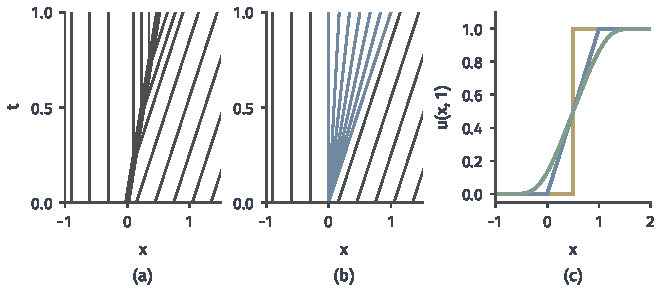
\includegraphics[width=112.0mm]{figures/06-differential-equations/02-partial-differential-equations/matplotlib/pdeprob-riemann/figure.pdf}
  \caption{同一台阶初值的两个弱解。(a)间断解：深灰粗线是间断线$x=t/2$，细线是特征线，它们都从间断线离开。(b)扇形解：蓝线是从原点发出的扇形特征线。(c)$t=1$的形状：间断解（黄）、扇形解（蓝）、带黏性$\nu=0.02$的数值解（绿）。}
  \label{fig:pdeprob-riemann}
\end{BookInlineFigure}

要恢复唯一性，就要在弱解中增加一条选择规则，只保留与小黏性极限一致的解。满足这种规则的弱解称为\term{熵解}（entropy solution），第~\ref{chap:scalar-conservation-laws}章给出精确的定义并证明唯一性。

\paragraph{Hamilton--Jacobi方程：几乎处处太宽}
最后一种情况说明，弱导数的办法并不总能用上。考虑$\lvert u'\rvert=1$，$x\in(-1,1)$，$u(\pm1)=0$，这是从边界出发、速度为$1$的波前的到达时间所满足的方程。

它没有$C^{1}$解。若$u\in C^{1}$，由Rolle定理存在一点$u'=0$，与$\lvert u'\rvert=1$矛盾。若只要求几乎处处成立，又有太多的解：图~\ref{fig:pdeprob-eikonal}(a)中每一条锯齿线的斜率都是$\pm1$，可以折任意多次。

这里不能把导数转到测试函数上，因为方程对$u'$非线性，$\lvert u'\rvert$无法通过分部积分移走。可行的选择办法仍然是加小黏性。考虑
\[
  (u')^{2}-\varepsilon u''=1,\qquad u(\pm1)=0.
\]
它有显式解
\begin{equation}
  u_\varepsilon(x)=\varepsilon\Bigl(\ln\cosh\frac{1}{\varepsilon}-\ln\cosh\frac{x}{\varepsilon}\Bigr).
  \label{eq:pdeprob-viscous-eikonal}
\end{equation}

下面验证。两次求导得到
\[
  u_\varepsilon'=-\tanh\frac{x}{\varepsilon},\qquad
  u_\varepsilon''=-\frac{1}{\varepsilon}\operatorname{sech}^{2}\frac{x}{\varepsilon}.
\]
于是
\[
  (u_\varepsilon')^{2}-\varepsilon u_\varepsilon''=\tanh^{2}\frac{x}{\varepsilon}+\operatorname{sech}^{2}\frac{x}{\varepsilon}=1.
\]
边值也满足，因为$\cosh$是偶函数。令$\varepsilon\to0$，由$\cosh s\approx\frac12\mathrm{e}^{\lvert s\rvert}$（$\lvert s\rvert$很大时），
\[
  \varepsilon\ln\cosh\frac{x}{\varepsilon}\to\lvert x\rvert,
\]
所以$u_\varepsilon\to1-\lvert x\rvert$。这正是到边界的距离，即波前的最短到达时间。图~\ref{fig:pdeprob-eikonal}(b)显示了这个极限。

\begin{BookInlineFigure}
  \centering
  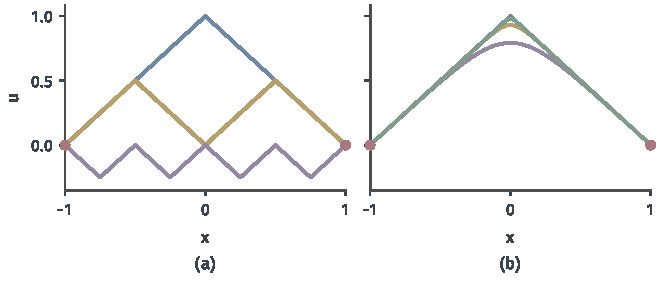
\includegraphics[width=112.0mm]{figures/06-differential-equations/02-partial-differential-equations/matplotlib/pdeprob-eikonal/figure.pdf}
  \caption{$\lvert u'\rvert=1$，$u(\pm1)=0$（红点）。(a)几个几乎处处满足方程的函数：$1-\lvert x\rvert$（蓝）和两条锯齿线（黄、紫）。(b)小黏性解$u_\varepsilon$，$\varepsilon=0.3$（紫）、$0.1$（黄）、$0.03$（绿）趋于$1-\lvert x\rvert$（蓝）。}
  \label{fig:pdeprob-eikonal}
\end{BookInlineFigure}

注意$\varepsilon$前的符号决定了选中的解：把$-\varepsilon u''$换成$+\varepsilon u''$，极限就成了$\lvert x\rvert-1$。这条选择规则的严格形式不用导数，而是在解被光滑函数从上方或下方触碰的点上提出不等式，满足它的解称为\term{黏性解}（viscosity solution），第~\ref{chap:hamilton-jacobi-equations}章专门讨论。

表~\ref{tab:pdeprob-solution-concepts}对比了这几种解的概念。它们不是彼此竞争的定义，而是针对不同方程结构的不同检验方式，光滑时都回到经典解。

\begin{BookInlineTable}
  \centering
  \begin{tabular}{lll}
    \toprule
    解的概念 & 检验方式 & 用在哪里\\
    \midrule
    经典解 & 逐点代入导数 & 数据和解都足够光滑\\
    弱解 & 导数转到测试函数上 & 方程有散度结构\\
    熵解 & 弱解，加熵条件 & 标量守恒律\\
    黏性解 & 用光滑函数从两侧触碰 & Hamilton--Jacobi方程\\
    \bottomrule
  \end{tabular}
  \caption{几种解的概念。}
  \label{tab:pdeprob-solution-concepts}
\end{BookInlineTable}
